In \autoref{abb:ProdukteDB} werden verwendbare Dienste für die datenbankseitige (\enquote{\ac{OLAP}} Verarbeitung) von \ac{AWS}, gemeinsam mit ihren jeweiligen Einsatzgebieten gezeigt. In diesem Abschnitt soll besonders auf die Dienste zur Verarbeitung nach dem Laden der Daten in eine der gezeigten Datenquellen eingegangen werden. Gezeigt werden jedoch auch Dienste für Datenvisualisierung und Machine Learning, da diese komplementär oder mit den prozessierten Daten verwendet werden können. Da die einzelnen Datenquellen jeweils verschiedene Sprachen, bzw. Dialekte von \ac{SQL} verwenden, sind die spezifischen Abfragesprachen mit einem generischen Eintrag in der Grafik abgebildet. Dabei ist es bei \ac{AWS} durchaus üblich, Interoperabilität zu anderen \ac{AWS} Diensten, wie beispielsweise Lambda, in den jeweiligen \ac{SQL} Dialekt einzubauen.

\begin{figure}[H]
\centering
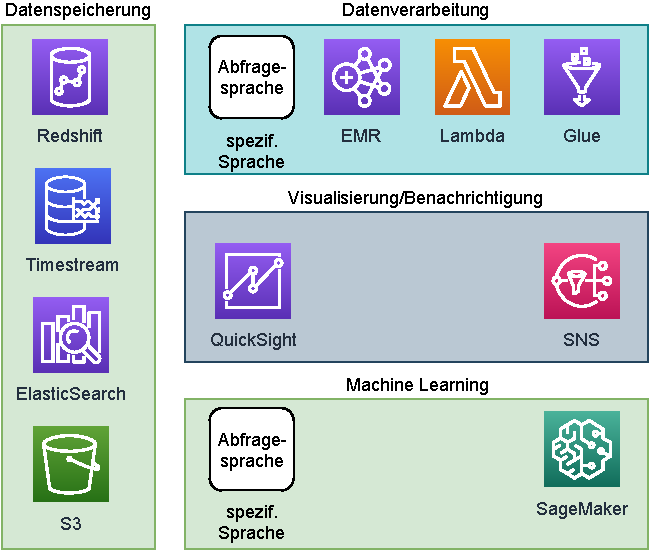
\includegraphics[width=\textwidth]{graphics/Overview-DB.pdf}
\caption{Einsetzbare Produkte im Bereich Datenbankverarbeitung}
\label{abb:ProdukteDB}
\end{figure}

\subsection{Amazon Timestream}



Timestream ist nach Aussage des Herstellers eine schneller, skalierbare und speziell für Zeitreihendaten entwickelte Datenbank, welche über \ac{AWS} als Dienstleistung bezogen werden kann.\footcite[Vgl. auch im Folgenden][]{AmazonWebServicesInc..o.J.h} Timestream integriert zwei verschiedene Speichertypen, nämlich \ac{RAM}-basierten Speicher, in dem Daten auf welche schnell zugegriffen werden sollen gespeichert werden können und Festplatten-basierten Speicher, welcher für historische Daten dienen soll.
Timestream besetzt zusätzlich einen eigenen \ac{SQL}-Dialekt, welcher um Funktionen zur Analyse von Zeitreihendaten erweitert wurde. Ein Beispiel für den Einsatz des \ac{SQL}-Dialekts zur Kalkulation des 99. Perzentils ist in \autoref{lst:sql-timestream} gezeigt.
\lstset{language=SQL} 

\begin{lstlisting}[caption={Berechnung des 99. Perzentils in Timestream},label=lst:sql-timestream, captionpos=b]
SELECT DeviceType,
  measure_name,
  BIN(time, 120m) AS binned_timestamp,
  ROUND(AVG(measure_value::double), 2) AS avg,
  ROUND(APPROX_PERCENTILE(measure_value::double, 0.99), 2) AS p99 
FROM "iot - demo".iot 
WHERE measure_name = 'temperature' 
  AND time > ago(24h) 
GROUP BY DeviceType,
  measure_name,
  BIN(time, 120m) 
ORDER BY ABS(avg - p99) DESC
\end{lstlisting}

\begin{table}[H]
\centering
\begin{tabular}{|l|l|l|l|l|}
\hline
DeviceType & measure\_name & binned\_timestamp & avg & p99 \\ \hline
iotDemo & temperature & 2021-02-26 08:00:00.000000000 & 16.51 & 20.1 \\ \hline
iotDemo & temperature & 2021-02-26 16:00:00.000000000 & 18.23 & 19.2 \\ \hline
iotDemo & temperature & 2021-02-25 18:00:00.000000000 & 18.5 & 19.3 \\ \hline
iotDemo & temperature & 2021-02-25 20:00:00.000000000 & 17.3 & 17.8 \\ \hline
\end{tabular}
\caption{Ausgabe der Datenbank bei Eingabe des oben gezeigten SQL-Statements}
\label{tab:AusgabeSQL}
\end{table}

\subsection{Amazon Redshift}
Amazon Redshift ist der Data Warehouse Dienst von \ac{AWS}, welcher nach Aussage des Herstellers \enquote{enterprise-level} ist und auf ein Datenvolument von Petabytes skalieren kann. \footcite[Vgl.][1]{AmazonWebServicesInc..o.J.g} Redshift ist dabei ein klassisches \ac{OLAP} Produkt, welches für eine Vielzahl verschiedener Daten effizient Auswertungen bereitstellen kann. Redshift basiert auf der bekannten Open Source Datenbank PostgreSQL, weicht jedoch in der Implementierung diverser Kommandos und Features ab, die das Amazon als irrelevant für \ac{OLAP} Anwendungen hält.\footcite[Vgl.][4]{AmazonWebServicesInc..o.J.g}\nzitat\footcite[Vgl.][428\psqq]{AmazonWebServicesInc..o.J.g} Kern von Redshift sind sogenannte Cluster, welche aus einer oder mehrerer Berechnungsknoten (\enquote{compute nodes}) und Anführerknoten(\enquote{leader nodes}) besteht. Applikationen interagieren allein mit den Anführerknoten, die existierenden Berechnungsknoten sind zwar transparent für die Anwendung, werden jedoch von den Anführerknoten mit Ausführungsplänen versorgt, die diese entwickelt um Anfragen effizient zu verarbeiten.\footcite[Vgl.][4]{AmazonWebServicesInc..o.J.g}

\subsection{Amazon S3}
Amazon \acf{S3} ist per se nur ein Datenspeicherungsdienst, wird jedoch von Amazon kombiniert mit dem Dienst AWS Lake Formation als Basis für einen Data Lake empfohlen.\footcite[Vgl.][]{AmazonWebServicesInc..o.J.f}\nzitat\footcite[Vgl.][2\psqq]{AmazonWebServicesInc..2017}

\subsection{Amazon Athena}
Amazon Athena ist nach Aussage des Herstellers ein voll verwalteter Query Dienst, welcher das durchsuchen von großen Datenmengen im \ac{S3} Speicherdienst möglich macht.\footcite[Vgl.][]{Barr.2016} Athena basiert dabei auf dem ursprünglich von Facebook entwickelten Presto, welches mittlerweile Open Source ist. Innerhalb von Athena können Daten verschiedener Formate (\ac{CSV}, Apache Parquet, Apache ORC, \ac{JSON}, ...) mittels \ac{SQL} verarbeitet werden.

\subsection{Amazon Elasticsearch}
Amazon Elasticsearch ist die verwaltetete Variante der ehemals Open-Source Elasticsearch Datenbank, entwickelt von Elastic.\footcite[Vgl.][]{Barr.01.10.2015} Elasticsearch ist dabei nach Aussage des Herstellers eine verteilte, freie und offene Analytics- und Suchplattform für viele verschiedenen Datenformen.\footcite[Vgl.][]{ElasticsearchInc..o.J.} Elasticsearch basiert auf der Open Source Bibliothek Apache Lucene. Elasticsearch geniesst neben der Popularität im Bereich Logverarbeitung und Monitoring auch Beliebtheit als \ac{IIoT} Datenbank.\footcite[Vgl.][]{Mantfeld.2019}\nzitat\footcite[Vgl.][]{Bajer.2017}



\subsection{Produktauswahl}